\chapter{Đánh giá hệ thống}\label{chap4}
Việc thực hiện đánh giá hệ thống sau khi đã triển khai trên môi trường thực nghiệm là một bước quan trọng giúp đảm bảo hệ thống hoạt động đúng như mong đợi, đáp ứng các yêu cầu về hiệu suất độ tin cậy và khả năng mở rộng.
Chương này sẽ đánh giá hiệu quả hoạt động thông qua các bộ kiểm thử được cấu hình sẵn.
Ngoài ra ở Chương này đề cập đến một số vấn đề gặp phải trong quá trình phát triển nên tảng quản lý quán ăn.
\section{Hiệu quả hoạt động}\label{sec:efficiency}
Để đánh giá hiệu quả hoạt động của hệ thống một cách toàn diện, hai bộ kiểm thử được tiến hành gồm kiểm thử tự động mở rộng và kiểm thử tính sẵn sàng cao.
Kiểm thử tự động mở rộng tập trung vào khả năng GKE tự động điều chỉnh tài nguyên, số lượng Node, Pod để đáp ứng với sự biến động trong lưu lượng truy cập.
Kiểm thử tính sẵn sàng cao sẽ đánh giá xem liệu hệ thống có thể duy trì hoạt động liên tục ngay cả khi gặp sự cố
\subsection{Kiểm thử tự động mở rộng}
Bằng việc sử dụng HPA của K8s trên môi trường đám mây của GCP, cấu hình phần cứng của các Pod được định nghĩa ở Đoạn mã~\ref{cod:storage-service-hardware}.
\tcode{limits} là cấu hình phần cứng tối đa (bộ nhớ và CPU) mà Pod đó được phép tiêu thụ.
Đây là giá trị ngưỡng cố định được đặt ra bởi K8s.
\tcode{requests} là số lượng bộ nhớ và CPU tối thiểu mà Pod yêu cầu để hoạt động và K8s sẽ đảm bảo lượng tài nguyên này sẽ luôn khả dụng cho Pod.
Theo cấu hình tại Dòng~\ref{line:sp}, Đoạn mã~\ref{cod:k8s-gitlab-ci/cd}, mỗi deployment sẽ có tối đa năm Pod hoạt động cùng lúc nhưng để phục vụ mục đích kiểm thử với lưu lượng thực tế của một hệ thống lớn, số lượng Pod tối đa đã được điều chỉnh lên 20 Pod.
Dịch vụ được chọn để chạy kiểm thử sẽ là dịch vụ lưu trữ tệp \tcode{storage-service}, dịch vụ này phụ trách việc lưu trữ ảnh và các tệp do người dùng tải lên một S3 bucket của AWS (Amazon Web Service).
API được gọi cho mục đích kiểm thử sẽ là một API lấy mã QR thanh toán của nhà hàng đã được tải lên S3.
\begin{lstlisting}[style=yaml, caption={Đoạn mã cấu hình phần cứng cho \tcode{storage-service} trên GKE.}, label={cod:storage-service-hardware},  captionpos=b]
resources:
    limits:
        cpu: 300m
        memory: 500Mi
    requests:
        cpu: 200m
        memory: 300Mi
\end{lstlisting}
\begin{figure}
    \centering
    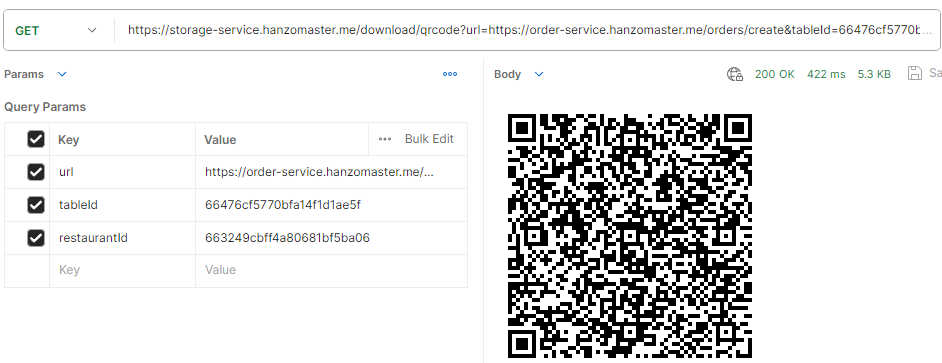
\includegraphics[width=1\linewidth]{images/hChip/test/API-example.png}
    \caption{API lấy mã QR thanh toán của nhà hàng, quán ăn}
    \label{fig:API-QR-code}
\end{figure}
\begin{figure}[H]
	\centering
	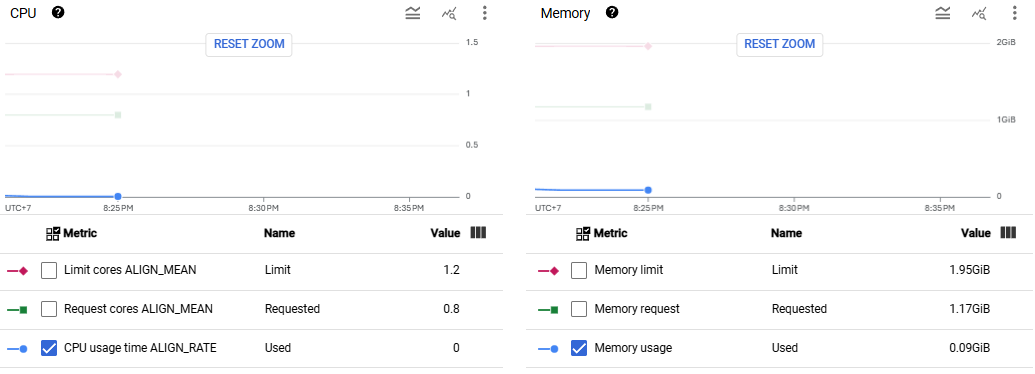
\includegraphics[width=\textwidth]{images/hChip/test/resourse-before-test.png}
	\caption{Lượng tài nguyên trước khi bắt đầu kiểm thử tự động mở rộng}
	\label{fig:resource-before-test}
\end{figure}
Hình~\ref{fig:resource-before-test} cho thấy lượng tài nguyên Deployment trước khi bắt đầu gọi API có số lượng bộ nhớ tối đa có thể truy cập được là \tcode{1.95GiB} tương đương với 4 Pod đang hoạt động.
Công cụ được sử dụng để chạy kiểm thử là Jmeter, một công cụ kiểm thử hiệu năng mã nguồn mở nổi tiếng thường xuyên được dùng trong các công việc liên quan đến đo lường và phân tích hiệu suất của cá ứng dụng web cũng như là các dịch vụ.
\begin{figure}
    \centering
    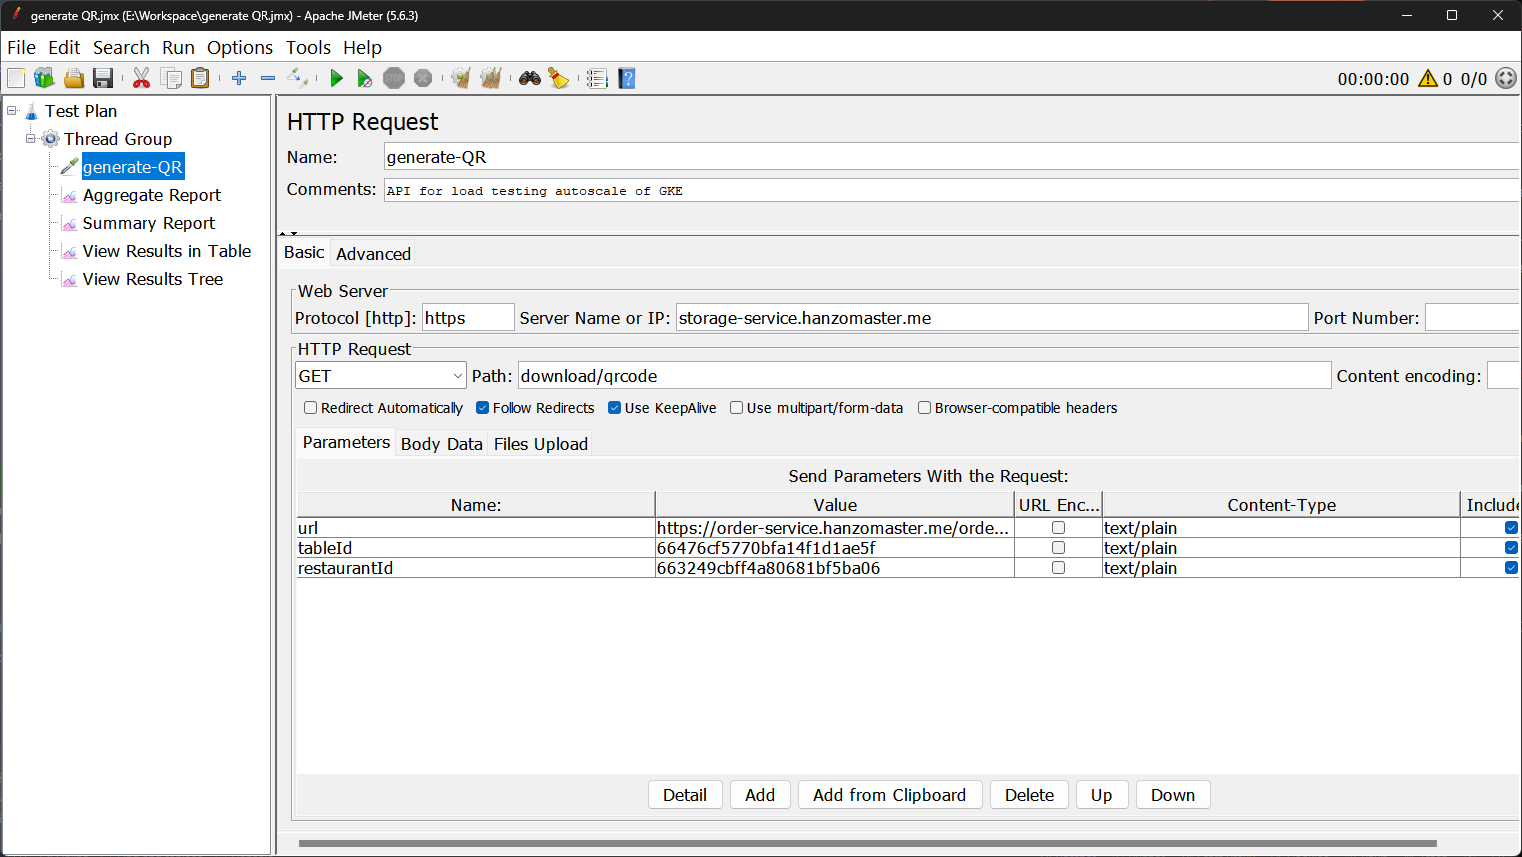
\includegraphics[width=1\linewidth]{images/hChip/test/Jmeter-setup.png}
    \caption{Bộ kiểm thử API của Jmeter}
    \label{fig:Jmeter-API}
\end{figure}
Cấu hình Jmeter chạy bộ kiểm thử API với 200 luồng tương đương với 200 người dùng và thời gian tăng trưởng (ramp-up period) 20 giây trong 15 phút, ta có được các chỉ số như sau.
\begin{figure}
    \centering
    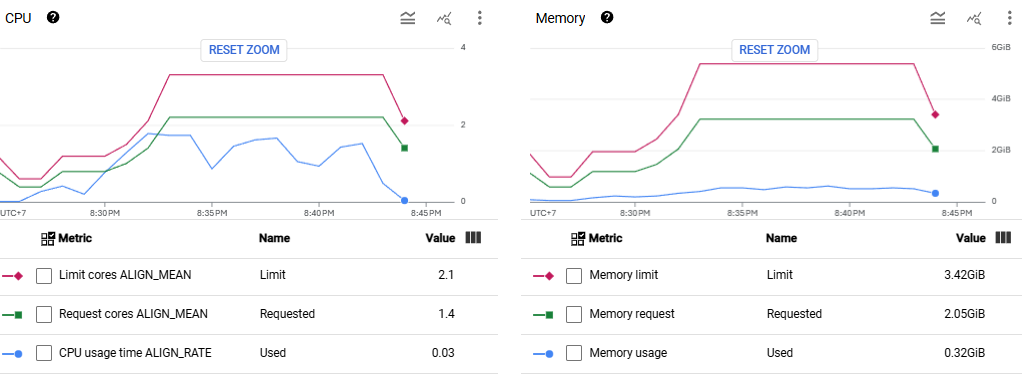
\includegraphics[width=1\linewidth]{images/hChip/test/resource-after-15m.png}
    \caption{Lượng tài nguyên sử dụng trong quá trình chạy Jemter kiểm tra tải}
    \label{fig:resource-after-15}
\end{figure}
Ở thời điểm số lượng lời gọi vào hệ thống nhiều nhất, hệ thống mở rộng lên tới 11 Pod và lượng tài nguyên được các Pod yêu cầu tiêu thụ là\tcode{3.22GiB}.
\begin{figure}
    \centering
    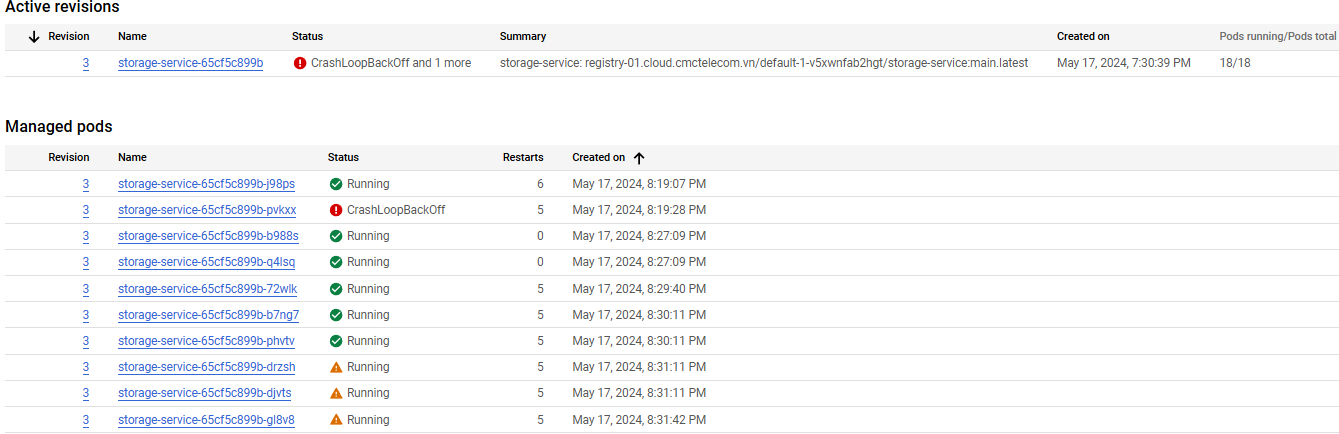
\includegraphics[width=1\linewidth]{images/hChip/test/pod-number-after-15m.png}
    \caption{Số lượng Pod trong quá trình chạy Jmeter kiểm tra tải}
    \label{fig:pod-number-after-15}
\end{figure}
Ngoài ra số lượng Node cũng được K8s cấu hình tăng cường lên trong quá trình này.
Một số Pod khi hệ thống hứng chịu một lượng yêu cầu lớn có biểu hiện lỗi do Pod dùng quá bộ nhớ giới hạn của K8s khiến cho Pod bị buộc tắt đi và bật lại.
Sau khi quá trình chạy Jmeter hoàn tất, các Pod đều trở lại hoạt động bình thường và K8s tự động giảm số lượng Node và Pod về cấu hình mặc định.
\subsection{Kiểm thử tính sẵn sàng cao}
Bộ kiểm thử này được sử dụng với mục tiêu xác định khả năng phục hồi của hệ thống khi gặp sự cố cũng như là tính sẵn sàng cao của hệ thống, tức khi một hệ thống không hoạt động thì các lời gọi yêu cầu đến vẫn có thể được xử lý tại một mức nhất định.
Có nhiều cách nhằm đảm bảo tính sẵn sàng cao của hệ thống, các phương pháp truyền thống vẫn hay được sử dụng như DC/DR (Data Center/Diaster Recovery) kèm theo cân bằng tải giúp giảm thiểu rủi ro khi một thành phần gặp sự cố.
Ngoài ra, việc sao lưu dữ liệu thường xuyên cũng là những biện pháp cần thiết giúp duy trì tính liên tục của dịch vụ.

Trong kiến trúc vi dịch vụ, việc sử dụng nhiều cụm K8s đã trở thành một giải pháp hiệu quả để duy trì HA.
Với cách tiếp cận này, ứng dụng sẽ được triển khai trên nhiều cụm K8s độc lập, phân tán trên các vùng địa lý khác nhau.
Khi một cụm gặp sự cố, lưu lượng truy cập sẽ được tự động chuyển hướng đến các cụm khác, đảm bảo tính liên tục của dịch vụ.
Trên thực tế, việc duy trì tính liên tục của hệ thống còn gặp nhiều khó khăn do vấn đề không chỉ nằm ở cụm K8s chạy các dịch vụ xử lý chính của hệ thống mà lỗi có thể rải rác ở bất cứ vị trí nào từ Cổng API, cân bằng tải của Clouflare, cơ sở dữ liệu MongoDB.
Ở mỗi vùng này ta đều cần có các biện pháp sao lưu, dự phòng phù hợp giúp tránh hệ thống gặp sự cố khiến cho dịch vụ ngừng hoạt động.

Hệ thống quản lý nhà hàng, quán ăn được cấu hình chia làm hai cụm chạy độc lập với nhau trên GKE của GCP.
Từ đó ta sẽ cấu hình Cổng API của Kong giúp cân bằng tải đến cả hai cụm.
Ở đây ta sẽ điều chỉnh thêm một Upstream mới với IP của máy chủ đích đến là cụm dự phòng của hệ thống với cùng một thông số \tcode{Weight}.
Điều này có nghĩa là lưu lượng truy cập sẽ được phân phối điều cho cả hai máy chủ.
\begin{figure}
    \centering
    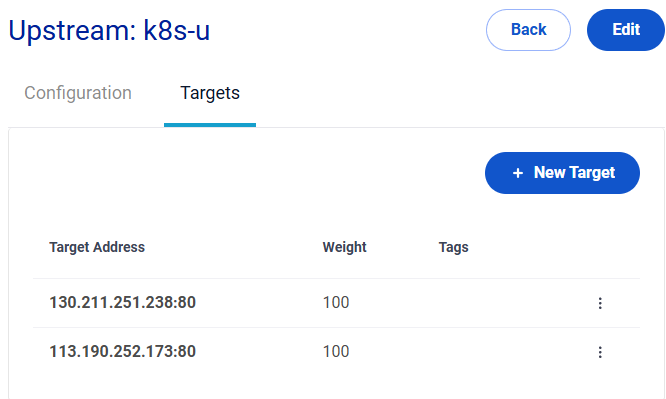
\includegraphics[width=1\linewidth]{images/hChip/test/kong-upstream.png}
    \caption{Các máy chủ được cấu hình trỏ đến trong Kong Gateway}
    \label{fig:kong-upstream}
\end{figure}
Sau khi đã cấu hình xong, giờ đây thông qua các API kiểm tra tình trạng của hệ thống (health check), Kong Gateway sẽ định kỳ gọi đến các API này nhằm phát hiện hệ thống có gặp phải sự cố hay không.
Khi một hệ thống bị đánh dấu là ngừng hoạt động, Kong Gateway sẽ ngừng chuyển hướng lưu lượng truy cập máy chủ đó mà chuyển các yêu cầu gọi API đến máy chủ còn đang hoạt động.
Khi máy chủ gặp sự cố nhận yêu cầu gọi trở lại, Kong Gateway sẽ tự động phát hiện thông qua API kiểm tra tình trạng hoạt động của hệ thống và chuyển hướng lưu lượng truy cập trở lại máy chủ đó.
Điều này giúp ứng dụng đạt tính sẵn sàng cao khi hạn chế được thời gian ngừng hoạt động của hệ thống bằng cách phân phối dữ liệu trên nhiều máy chủ khác nhau.